\documentclass{article}

\usepackage{ctex}
\usepackage{anyfontsize}
\usepackage{amsfonts}
\usepackage{amsmath}
\usepackage{amsthm}
\usepackage{graphicx}
\usepackage{float}
\usepackage{hyperref}
\usepackage{mathabx}
\usepackage{datetime}
\usepackage{tabularray}
\usepackage{mathrsfs}
\usepackage{geometry}
\usepackage{pdflscape}
\usepackage{tikz}
\usepackage{pgfplots}

\title{概率论与数理统计}
\author{}
\date{\today}

\geometry{a4paper,scale=0.8}

\begin{document}

\hypersetup{
    hidelinks,
    %colorlinks = true,
    allcolors = black,
    %pdfstartview = Fit,
    breaklinks = true
}

\newtheorem{definition}{Definition}[subsubsection]
\newtheorem{theorem}{Theorem}[subsubsection]
\newtheorem{corollary}{Corollary}[theorem]
\renewcommand{\proofname}{\indent\bf Proof}
\numberwithin{equation}{subsection}

\def\e{\mathrm e}
\def\i{\mathrm i}
\def\j{\mathrm j}
\def\d{\mathrm d}
\def\C{\mathrm C}
\def\sr{\mathbb R}
\def\sn{\mathbb N}
\def\snp{\mathbb N^+}
\def\sc{\mathbb C}
\def\sz{\mathbb Z}
\def\impint{\int\limits_{-\infty}^{+\infty}}

\newcommand{\abs}[1]{\left|#1\right|}
\newcommand{\p}[1]{\left(#1\right)}
\newcommand{\B}[1]{\left\{#1\right\}}
\newcommand{\conditionset}[2]{\B{#1|#2}}
\newcommand{\cov}[2]{\mathrm{Cov}\p{#1,#2}}

\def\pa{P\p{A}}
\def\sumin{\sum\limits_{i=1}^n}

\begin{titlepage}
    \maketitle
\end{titlepage}

\tableofcontents
\newpage

\part{概率论}

\section{随机事件及其概率}

\subsection{符号}

\begin{center}
    \begin{tblr}{c|c|c}
        \hline
        名词     & 符号             & 注释                                                     \\
        \hline
        随机实验   & $E$            &                                                        \\
        样本点    & $\omega$       &                                                        \\
        样本空间   & $\Omega$       &                                                        \\
        交(积)事件 & $A\cap B$或$AB$ & $\conditionset\omega{\omega\in A\wedge\omega\in B}$    \\
        并事件    & $A\cup B$      & $\conditionset\omega{\omega\in A\vee\omega\in B}$      \\
        差事件    & $A-B$          & $\conditionset\omega{\omega\in A\wedge\omega\notin B}$ \\
        相容事件   &                & $A\cap B\neq\emptyset$                                 \\
        互斥事件   &                & $A\cap B=\emptyset$                                    \\
        对立事件   & $\overline A$  & $\Omega-A$                                             \\
        概率     & $\pa$          &                                                        \\
        \hline
    \end{tblr}
\end{center}

\subsection{条件概率}

已知$A$事件发生,发生$B$事件的概率($\pa>0$)

\[P\p{B|A}=\frac{P\p{AB}}{\pa}\]

\subsection{乘法公式}

$\pa>0$

\[P\p{AB}=\pa P\p{B|A}\]

\subsection{古典概型}

\[\pa=\frac{A\text{所含样本点个数}}{\Omega\text{样本点个数}}\]

\subsection{几何概型}

\[\pa=\frac{A\text{的几何测度}}{\Omega\text{的几何测度}}\]

\subsection{完备事件组}

$\B{A_i}$

\[\bigcup A_i=\Omega;A_i\cap A_j=\emptyset\p{i\neq j}\]

\subsection{全概率公式}

\begin{enumerate}
    \item [$\B{A_i}$] 完备事件组
\end{enumerate}

\[P\p{B}=\sum P\p{A_iB}=\sum P\p{A_i}P\p{B|A_i}\]

\subsubsection{全概率条件公式}

\[P\p{C|B}=\sum P\p{A_iC|B}=\sum P\p{A_i|B}P\p{C|A_iB}\]

\subsection{贝叶斯公式}

\[P\p{A_j|B}=\frac{P\p{A_jB}}{P\p{B}}
    =\frac{P\p{A_jB}}{\sum P\p{A_iB}}
    =\frac{P\p{A_j}P\p{B|A_j}}{\sum P\p{A_i}P\p{B|A_i}}\]

\subsection{独立事件}

\[\begin{aligned}
        A,B\text{相互独立} & \iff P\p{AB}=\pa P\p{B}                \\
                       & \iff P\p{A|B}=\pa                      \\
                       & \iff P\p{A|B}=P\p{A|\overline B}       \\
                       & \iff\overline A,B\text{相互独立}           \\
                       & \iff A,\overline B\text{相互独立}          \\
                       & \iff\overline A,\overline B\text{相互独立}
    \end{aligned}\]

\[\begin{aligned}
        A,B,C\text{相互独立}\iff & P\p{AB}=\pa P\p{B};       \\
                             & P\p{AC}=\pa P\p{C};       \\
                             & P\p{BC}=\pa P\p{C};       \\
                             & P\p{ABC}=\pa P\p{B}P\p{C}
    \end{aligned}\]

\subsection{伯努利概型}

定义:
\begin{enumerate}
    \item 每次试验对应样本空间相同
    \item 各次试验结果相对独立
    \item 只考虑两种结果
\end{enumerate}

$n$重伯努利试验中,$A$事件恰好发生$k$次的概率为$\C_n^kp^k\p{1-p}^{n-k}$

\section{连续型随机变量及其分布函数}

\subsection{密度函数(概率密度)}

$f\p{x}$、$f\p{x,y}$等

\paragraph{性质}

\[f\p{x}\geqslant0\]

\[\impint f\p{x}\d x=1\]

\[\impint\impint f\p{x,y}\d x\d y=1\]

\subsection{分布函数}

$F\p{x}$、$F\p{x,y}$等

\paragraph{定义}

\[P\B{X=x_0}=\lim_{x\to x_0^+}F\p{x}-\lim_{x\to x_0^-}F\p{x}\]

当$F\p{x}$连续时(连续型随机变量)

\[P\B{X=x_0}=0\]

\[F\p{x}=P\B{X\leqslant x}=\int\limits_{-\infty}^xf\p{t}\d t\]

\[F\p{x,y}=P\B{X\leqslant x,Y\leqslant y}=\int\limits_{-\infty}^x\int\limits_{-\infty}^yf\p{u,v}\d u\d v\]

\paragraph{性质}

\[F\p{x}\geqslant0\]

\[\lim_{x\to+\infty}F\p{x}=1\]

\section{分布}

\subsection{边缘分布}

\[F_X\p{x}=P\B{X\leqslant x}=\lim_{y\to+\infty}F\p{x,y}=F\p{x,+\infty}\]

\[F_Y\p{y}=P\B{Y\leqslant y}=\lim_{x\to+\infty}F\p{x,y}=F\p{+\infty,y}\]

\subsubsection{边缘分布律}

\[P\B{X=x_i}=\sum_jP\B{X=x_i,Y=y_j}\]

\[P\B{Y=y_j}=\sum_iP\B{X=x_i,Y=y_j}\]

\subsubsection{边缘密度函数}

\[f_X\p{x}=\impint f\p{x,y}\d y\]

\[f_Y\p{y}=\impint f\p{x,y}\d x\]

\subsection{条件分布}

\[F_{X|Y}\p{x|y}=P\B{X\leqslant x|Y=y}=\int\limits_{-\infty}^x f_{X|Y}\p{t|y}\d t\]

\[F_{Y|X}\p{y|x}=P\B{Y\leqslant y|X=x}=\int\limits_{-\infty}^y f_{Y|X}\p{x|t}\d t\]

\subsubsection{条件分布律}

\[p_{j|i}=P\B{Y=y_j|X=x_i}=\frac{P\B{X=x_i,Y=y_j}}{P\B{X=x_i}}=\frac{p_{ij}}{p_{i\cdot}}\]

\[p_{i|j}=P\B{X=x_i|Y=y_j}=\frac{P\B{X=x_i,Y=y_j}}{P\B{Y=y_j}}=\frac{p_{ij}}{p_{\cdot j}}\]

\subsubsection{条件密度函数}

\[f_{X|Y}\p{x|y}=\frac{f\p{x,y}}{f_Y\p{y}}\]

\[f_{Y|X}\p{y|x}=\frac{f\p{x,y}}{f_X\p{x}}\]

\subsection{独立性}

\[\p{X,Y}\sim f\p{x,y}\]

若$X,Y$独立

充要条件1:

\[f\p{x,y}=f_X\p{x}f_Y\p{y}\]

充要条件2:

\[F\p{x,y}=F_X\p{x}F_Y\p{y}\]

\subsection{换元}

以下都有

\[\p{X,Y}\sim f\p{x,y}\]

其中$g$为单调可导函数

\subsubsection{一维}

$Y=h\p{X}$

令$g=h^{-1}$,即$X=g\p{Y}$,其中$g$为单调可导函数(即$h$的反函数单调可导)

\[\begin{aligned}
        F_Y\p{y} & =P\B{Y\leqslant y}                                                      \\
                 & =P\B{h\p{X}\leqslant y}                    &  & =P\B{X\leqslant g\p{y}} \\
                 & =F_{h\p{X}}\p{y}                           &  & =F_X\p{g\p{y}}          \\
                 & =\int\limits_{h\p{X}\leqslant y}f\p{t}\d t
    \end{aligned}\]

\[f_Y\p{y}=F_Y^\prime\p{y}\]

\subsubsection{二维}

$Z=g\p{X,Y}$

\[\begin{aligned}
        F_Z\p{z}             & =P\B{Z\leqslant z}                                   \\
                             & =P\B{g\p{X,Y}\leqslant z}                            \\
                             & =F_{g\p{X,Y}}\p{z}                                   \\
                             & =\iint_{g\p{X,Y}\leqslant z}f\p{u,v}\d u\d v         \\
        \text{若}X,Y\text{独立} & =\iint_{g\p{X,Y}\leqslant z}f_X\p{u}f_Y\p{v}\d u\d v
    \end{aligned}\]

\[f_Z\p{z}=F_Z^\prime\p{z}\]

\subsubsection{*和}

$Z=X+Y$

\[f_Z\p{z}
    =\impint f\p{x,z-x}\d x
    =\impint f\p{z-y,y}\d y\]

若$X,Y$独立

\[f_Z\p{z}
    =\impint f_X\p{x}f_Y\p{z-x}\d x
    =\impint f_X\p{z-y}f_Y\p{y}\d y
    =f_X\p{z}\ast f_Y\p{z}\]

\subsubsection{*商}

$Z=\dfrac XY$

\[f_Z\p{z}
    =\impint\abs yf\p{yz,y}\d y\]

若$X,Y$独立

\[f_Z\p{z}
    =\impint\abs yf_X\p{yz}f_Y\p{y}\d y\]

\subsubsection{*积}

$Z=XY$

\[f_Z\p{z}
    =\impint\frac1{\abs x}f\p{x,\frac zx}\d x
    =\impint\frac1{\abs y}f\p{\frac zy,y}\d y\]

若$X,Y$独立

\[f_Z\p{z}
    =\impint\frac1{\abs x}f_X\p{x}f_Y\p{\frac zx}\d x
    =\impint\frac1{\abs y}f_X\p{\frac zy}f_Y\p{y}\d y\]

\subsubsection{*最值分布}

若$X,Y$独立

\[M=\max\B{X,Y},N=\min\B{X,Y}\]

则

\[\begin{gathered}
        F_M=F_XF_Y\\
        1-F_N=\p{1-F_X}\p{1-F_Y}\\
        f_M=F^\prime_M=f_XF_Y+f_YF_X\\
        f_N=F^\prime_N=f_X\p{1-F_Y}+f_Y\p{1-F_X}
    \end{gathered}\]


\section{一维离散型随机变量及其分布律}

以下都有

\[p\in\p{0,1}\]

\subsection{两点分布}

$X\sim B\p{1,p}$

\[\begin{tblr}{c|c|c}
        \hline
        X & 0   & 1 \\
        \hline
        P & 1-p & p \\
        \hline
    \end{tblr}\]

\subsection{二项(伯努利)分布}

$X\sim B\p{n,p}$

\begin{enumerate}
    \item [$n$] $\in\snp$
    \item [$k$] $\geqslant k\in\sn$
\end{enumerate}

\[P\B{X=k}=\C_n^kp^k{\p{1-p}}^{n-k}\]

\subsection{泊松分布}

$X\sim P\p{\lambda}$

\begin{enumerate}
    \item [$\lambda$] $>0$
    \item [$k$] $\in\sn$
\end{enumerate}

\[P\B{X=k}=\frac{\lambda^k}{k!}\e^{-\lambda}\]

\subsubsection{泊松定理}

$n$重伯努利试验中,事件发生概率$p_n\in\p{0,1}$与试验次数有关,
当$p_n<0.1;n>100$时可近似为泊松分布。
若$\lim\limits_{n\to\infty}np_n=\lambda$,则

\[\lim_{n\to\infty}\C_n^kp_n^k\p{1-p_n}^{n-k}
    =\dfrac{\lambda^k}{k!}\e^{-\lambda}\]

$n$重伯努利试验:只有两种结果,且每次实验概率相同、相互独立,做$n$次

\subsection{几何分布}

$X\sim G\p{p}$

\begin{enumerate}
    \item [$k$] 前$k-1$次都失败,第$k$次成功$k\in\snp$
\end{enumerate}

\[P\B{X=k}={\p{1-p}}^{k-1}p\]

\subsection{超几何分布}

$X\sim H\p{M,N,n}$

\begin{enumerate}
    \item [$N$] $>1$总样本数
    \item [$n$] $\leqslant N$抽取样本数
    \item [$M$] $\leqslant N$指定样本数
    \item [$k$] $\in\sn\cap\left[\max\B{0,n+M-N},\min\B{M,n}\right]$抽到指定样本数
\end{enumerate}

\[P\B{X=k}=\frac{\C_M^k\C_{N-M}^{n-k}}{\C_N^n}\]

\section{一维连续型随机变量及其密度、分布函数}

\subsection{均匀分布}

$X\sim U\left[a,b\right]$

\[f\p{x}=\left\{\begin{aligned}
         & \frac1{b-a} &  & x\in\p{a,b}                                          \\
         & 0           &  & x\in\left(-\infty,a\right]\cup\left[b,+\infty\right)
    \end{aligned}\right.\]

\[F\p{x}=\left\{\begin{aligned}
         & 0               &  & x\leqslant a \\
         & \frac{x-a}{b-a} &  & x\in\p{a,b}  \\
         & 1               &  & x\geqslant b
    \end{aligned}\right.\]

\subsection{指数分布}

$X\sim E\p{\lambda}$

\begin{enumerate}
    \item [$\lambda$] $>0$
\end{enumerate}

\[f\p{x}=\left\{\begin{aligned}
         & \lambda\e^{-\lambda x} &  & x>0         \\
         & 0                      &  & x\leqslant0
    \end{aligned}\right.\]

\[F\p{x}=\left\{\begin{aligned}
         & 1-\e^{-\lambda x} &  & x>0         \\
         & 0                 &  & x\leqslant0
    \end{aligned}\right.\]

\subsection{正态(高斯)分布}

$X\sim N\p{\mu,\sigma^2}$

\begin{enumerate}
    \item [$\mu$] $\in\sr$ 期望
    \item [$\sigma$] $>0$ 标准差
\end{enumerate}

\[f\p{x}=\frac1{\sqrt{2\pi}\sigma}\exp\p{-\frac{{\p{x-\mu}}^2}{2\sigma^2}}\]

\[\Phi\p{x}=\frac12\mathrm{erf}\p{\frac{x-\mu}{\sqrt2\sigma}}+\frac12\]

\[Z=\frac{X-\mu}\sigma\sim N\p{0,1}\]

\subsubsection{标准正态分布}

$X\sim N\p{0,1}$

\begin{center}
    \begin{tikzpicture}
        \begin{axis}[
                axis lines=middle,
                %grid,
                %thick,
                domain=-4:4,
                xmin=-4,
                xmax=4,
                ymin=-0.1,
                ymax=0.5,
                %legend pos=outer north east,
                smooth,
            ]
            \addplot[
                domain=-4:4,
                samples=50,
                blue,
                thick]
            {exp(-x^2/2)/(2*pi)^(1/2)};
        \end{axis}
    \end{tikzpicture}
\end{center}

\[\varphi\p{x}=\frac1{\sqrt{2\pi}}\exp\p{-\frac{x^2}2}\]

\[\Phi_0\p{x}=\frac12\mathrm{erf}\p{\frac x{\sqrt2}}+\frac12\]

\subsubsection{经验原则}

\[P\B{\abs{X-\mu}<k\sigma}=2\Phi_0\p{k}-1\p{k\geqslant0}\]

\[\left\{\begin{aligned}
        P\B{\abs{X-\mu}<\enspace\sigma}=0.6827 \\
        P\B{\abs{X-\mu}<2\sigma}=0.9545        \\
        P\B{\abs{X-\mu}<3\sigma}=0.9973
    \end{aligned}\right.\]

\section{二维连续型随机变量及其密度函数}

\subsection{均匀分布}

$\p{X,Y}\sim U\p{D}$

\[f\p{x,y}=\left\{\begin{aligned}
         & \frac1{S_D} &  & \p{x,y}\in D    \\
         & 0           &  & \p{x,y}\notin D \\
    \end{aligned}\right.\]

\subsection{正态分布}

$\p{X,Y}\sim N\p{\mu_X,\mu_Y,\sigma_X^2,\sigma_Y^2,\rho}$

\begin{enumerate}
    \item [$\mu$] $\in\sr$ 期望
    \item [$\sigma$] $>0$ 标准差
    \item [$\rho$] $\in\p{-1,1}$,相关系数($\rho=0$时$X,Y$独立)
\end{enumerate}

\[f\p{x,y}=\frac1{2\pi\sigma_X\sigma_Y\sqrt{1-\rho^2}}
    \exp\left[-\frac1{2\p{1-\rho^2}}
        \p{\frac{{\p{x-\mu_X}}^2}{\sigma_X^2}
            -2\rho\frac{\p{x-\mu_X}\p{y-\mu_Y}}{\sigma_X\sigma_Y}
            +\frac{{\p{y-\mu_Y}}^2}{\sigma_Y^2}}\right]\]

若$X,Y$独立

\[\left.\begin{aligned}
        X\sim N\p{\mu_X,\sigma_X^2} \\
        Y\sim N\p{\mu_Y,\sigma_Y^2}
    \end{aligned}\right\}\implies
    \p{X,Y}\sim N\p{\mu_X,\mu_Y,\sigma_X^2,\sigma_Y^2,0}\]


\[Z=aX+bY\sim N\p{a\mu_X+b\mu_Y,a^2\sigma_X^2+b^2\sigma_Y^2}\]

\part{数理统计}

\section{数字特征}

\subsection{期望}

\[\begin{tblr}{c|c|c}
        \hline
                             & \text{离散型}                                  & \text{连续型}                                           \\
        \hline
        E\p{X}               & \displaystyle\sum x_ip_i                    & \displaystyle\impint xf\p{x}\d x                     \\
        E\p{Y}\p{Y=g\p{X}}   & \displaystyle\sum g\p{x_i}p_i               & \displaystyle\impint g\p{x}f\p{x}\d x                \\
        E\p{Z}\p{Z=g\p{X,Y}} & \displaystyle\sum_i\sum_jg\p{x_i,y_j}p_{ij} & \displaystyle\impint\impint g\p{x,y}f\p{x,y}\d x\d y \\
        \hline
    \end{tblr}\]

\subsubsection{性质}

\paragraph{线性}

\[E\p{kX+c}=kE\p{X}+c\]

\[E\p{X\pm Y}=E\p{X}\pm E\p{Y}\]

\paragraph{线性相关性}

\[X,Y\text{不相关}\iff E\p{XY}=E\p{X}E\p{Y}\]

\subsection{方差}

\[D\p{X}=E\left[\p{X-E\p{X}}^2\right]=E\p{X^2}-{\p{E\p{X}}}^2\]

\subsubsection{标准差}

\[\sqrt{D\p{X}}\]

\subsubsection{离散型}

\[D\p{X}=\sum{\p{x_i-E\p{X}}}^2p_i\]

\subsubsection{连续型}

\[D\p{X}=\impint{\p{x-E\p{X}}}^2f\p{x}\d x\]

\subsubsection{性质}

\paragraph{线性}

\[D\p{kX+c}=k^2D\p{X}\]

\paragraph{线性相关性}

\[X,Y\text{不相关}\iff D\p{X\pm Y}=D\p{X}+D\p{Y}\]

\subsection{标准化随机变量}

\[\begin{gathered}
        X^\ast=\frac{X-E\p{X}}{\sqrt{D\p{X}}}\\
        E\p{X^\ast}=0\\
        D\p{X^\ast}=1
    \end{gathered}\]

\subsection{常见分布期望方差}

\[\begin{tblr}{c|c|c}
        \hline
        X\sim F\p{X}      & E\p{X}         & D\p{X}                                              \\
        \hline
        B\p{n,p}          & np             & np\p{1-p}                                           \\
        P\p{\lambda}      & \lambda        & \lambda                                             \\
        G\p{p}            & \dfrac1p       & \dfrac{\p{1-p}}{p^2}                                \\
        H\p{M,N,n}        & \dfrac{nM}N    & n\cdot\dfrac MN\p{1-\dfrac MN}\cdot\dfrac{N-n}{N-1} \\
        \hline
        U\left[a,b\right] & \dfrac{a+b}2   & \dfrac{{\p{b-a}}^2}{12}                             \\
        E\p{\lambda}      & \dfrac1\lambda & \dfrac1{\lambda^2}                                  \\
        N\p{\mu,\sigma^2} & \mu            & \sigma^2                                            \\
        \hline
    \end{tblr}\]

\subsection{协方差}

\[\cov XY=E\left[\p{X-E\p{X}}\p{Y-E\p{Y}}\right]=E\p{XY}-E\p{X}E\p{Y}\]

\subsubsection{性质}

\[D\p{X\pm Y}=D\p{X}+D\p{Y}\pm2\cov XY\]

\[\cov XX=D\p{X}\]

\paragraph{交换律}

\[\cov XY=\cov YX\]

\paragraph{线性}

\[\cov Xc=0\]

\[\cov{\sum a_iX_i}{\sum b_jY_j}=\sum_i\sum_ja_ib_j\cov{X_i}{Y_j}\]

\subsubsection{协方差矩阵(对称矩阵)}

$X,Y$的协方差矩阵为

\[\begin{bmatrix}
        \cov XX & \cov XY \\
        \cov YX & \cov YY
    \end{bmatrix}=
    \begin{bmatrix}
        D\p{X}  & \cov XY \\
        \cov XY & D\p{Y}
    \end{bmatrix}\]

\subsection{(线性)相关系数}

\subsubsection{*(线性)均方误差}

用$aX+b$去拟合$Y$

\begin{enumerate}
    \item [$e\p{a,b}$] 越小表明线性关系越强,越大越弱
    \item [$e\p{a_0,b_0}$] 最小均方误差
    \item [$\p{a_0,b_0}$] 驻点
    \item [$a_0$] $\dfrac{\cov XY}{D\p{X}}$
    \item [$b_0$] $E\p{Y}-a_0E\p{X}$
\end{enumerate}

\[e\p{a,b}=E\left[{\p{Y-\p{aX+b}}}^2\right]\]

\[e\p{a_0,b_0}=\p{1-\rho^2_{XY}}D\p{Y}\]

\subsubsection{定义}

\[\rho_{XY}=\frac{\cov XY}{\sqrt{D\p{X}}\sqrt{D\p{Y}}}\]

\subsubsection{性质}

\[\rho\in\left[-1,1\right]\]

\[\abs{\rho_{XY}}=1\iff P\B{Y=aX+b}=1\p{a\neq0}
    \left\{\begin{aligned}
        a>0 &  & \text{(正相关)} & \rho_{XY}= & 1  \\
        a<0 &  & \text{(负相关)} & \rho_{XY}= & -1 \\
    \end{aligned}\right.\]

\[\rho_{\p{aX}\p{bY}}=\frac{ab}{\abs{ab}}\rho_{XY}\]

\subsubsection{不(线性)相关}

\[\begin{aligned}
             & \rho=0                    \\
        \iff & \cov XY=0                 \\
        \iff & E\p{XY}=E\p{X}E\p{Y}      \\
        \iff & D\p{X\pm Y}=D\p{X}+D\p{Y}
    \end{aligned}\]

独立$\implies$不相关

\section{大数定律与中心极限定理}

\subsection{切比雪夫不等式}

设$X$有有限方差(即有界)

\[\begin{aligned}
                 & \exists E\p{X},D\p{X};\forall\varepsilon>0                                   \\
        \to      & P\B{\abs{X-E\p{X}}\geqslant\varepsilon}\leqslant\frac{D\p{X}}{\varepsilon^2} \\
        \text{或} & P\B{\abs{X-E\p{X}}<\varepsilon}\geqslant1-\frac{D\p{X}}{\varepsilon^2}
    \end{aligned}\]

\subsection{大数定律}

\subsubsection{依概率收敛}

随机变量序列$\B{X_n}$依概率收敛于常数$a$

\[X_n\overset{P}{\to}a\p{n\to\infty}\]

定义为

\[\forall\varepsilon>0\to\lim_{n\to\infty}P\B{\abs{X_n-a}<\varepsilon}=1\]

\subsubsection{伯努利大数定律}

设事件$A$每次实验发生概率为$p$,且$n$重伯努利试验中发生次数为$n_A$,则

\[\begin{aligned}
                 & \forall\varepsilon>0                                            \\
        \to      & \lim_{n\to\infty}P\B{\abs{\frac{n_A}n-p}<\varepsilon}=1         \\
        \text{或} & \lim_{n\to\infty}P\B{\abs{\frac{n_A}n-p}\geqslant\varepsilon}=0
    \end{aligned}\]

\subsubsection{切比雪夫大数定律}

设随机变量序列$\B{X_i}$相互独立,且有有限方差,则

\[\begin{aligned}
                 & \forall\varepsilon>0                                                \\
        \to      & \lim_{n\to\infty}\B{\abs{\bar X-E\p{\bar X}}<\varepsilon}=1         \\
        \text{或} & \lim_{n\to\infty}\B{\abs{\bar X-E\p{\bar X}}\geqslant\varepsilon}=0
    \end{aligned}\]

\subsubsection{辛钦大数定律}

设随机变量序列$\B{X_i}$独立同分布,则有相同的期望$\mu$,则

\[\begin{aligned}
                 & \forall\varepsilon>0                                        \\
        \to      & \lim_{n\to\infty}\B{\abs{\bar X-\mu}<\varepsilon}=1         \\
        \text{或} & \lim_{n\to\infty}\B{\abs{\bar X-\mu}\geqslant\varepsilon}=0
    \end{aligned}\]

\subsection{中心极限定理}

\subsubsection{定理}

设随机变量序列$\B{X_i}$相互独立,期望、方差均存在,则

\[\lim_{n\to\infty}\sumin X_i\sim N\p{E\p{\sumin X_i},D\p{\sumin X_i}}\]

\[\lim_{n\to\infty}\frac{\sumin X_i-E\p{\sumin X_i}}{\sqrt{D\p{\sumin X_i}}}\sim N\p{0,1}\]

\[\lim_{n\to\infty}P\B{\frac{\sumin X_i-E\p{\sumin X_i}}{\sqrt{D\p{\sumin X_i}}}\leqslant x}=\Phi_0\p{x}\]

\subsubsection{列维-林德伯格定理(独立同分布)}

设随机变量序列$\B{X_i}$独立同分布,存在相同的期望$\mu$、方差$\sigma^2$,则

\[\lim_{n\to\infty}\sumin X_i\sim N\p{n\mu,n\sigma^2}\]

\[\lim_{n\to\infty}\frac{\sumin X_i-n\mu}{\sqrt n\sigma}\sim N\p{0,1}\]

\[\lim_{n\to\infty}P\B{\frac{\sumin X_i-n\mu}{\sqrt n\sigma}\leqslant x}=\Phi_0\p{x}\]

\subsubsection{棣莫弗-拉普拉斯定理(二项分布)}

设随机变量$\eta_n\sim B\p{n,p}$,则

\[\lim_{n\to\infty}\eta_n\sim N\p{np,np\p{1-p}}\]

\[\lim_{n\to\infty}\frac{\eta_n-np}{\sqrt{np\p{1-p}}}\sim N\p{0,1}\]

\[\lim_{n\to\infty}P\B{\frac{\eta_n-np}{\sqrt{np\p{1-p}}}\leqslant x}=\Phi_0\p{x}\]

显然$\eta_n=\sumin X_i$,其中随机变量序列$\B{X_i}$独立同服从$B\p{1,p}$分布

\section{统计量}

\subsection{样本容量}

\[n\]

\subsection{简单随机样本}

\[X_1,X_2,\cdots,X_n\text{相互独立且同分布}\]

\subsection{样本联合分布函数}

\[F\p{x_1,x_2,\cdots,x_n}=\prod F\p{x_i}\]

\[f\p{x_1,x_2,\cdots,x_n}=\prod f\p{x_i}\]

\[P\B{X_1=x_1,X_2=x_2,\cdots,X_n=x_n}=\prod p_i\]

\subsection{样本均值}

\[\bar X=\frac1n\sumin X_i\]

\subsection{(修正)样本方差}

\[S^2=\frac1{n-1}\sumin{\p{X_i-\bar X}}^2=\frac1{n-1}\p{\sumin X_i^2-n\bar X^2}\]

\subsection{样本标准差}

\[S=\sqrt{S^2}\]

\subsection{极差}

\[\max_{1\leqslant i\leqslant n}X_i-\min_{1\leqslant i\leqslant n}X_i\]

\subsection{其他}

样本均值的期望等于总体均值(期望),样本方差的期望等于总体方差

\[E\p{\bar X}=\mu=E\p{X}\]

\[E\p{S^2}=\sigma^2=D\p{X}\]

\[D\p{\bar X}=\frac{\sigma^2}n\]

\subsection{矩}

\[\begin{tblr}[
            note{$\ast$} = {$S_\omega=\sqrt{\dfrac{\p{m-1}S_X^2+\p{n-1}S_Y^2}{m+n-2}}$},
        ]{c|c|c|c}
        \hline
        \text{名称}        & \text{定义}                                      & \text{离散}                            & \text{连续}                                    \\
        \hline
        k\text{阶原点矩}     & E\p{X^k}                                       & \displaystyle\sum x_i^kp_i           & \displaystyle\impint x^kf\p{x}\d x           \\
        k\text{阶中心矩}     & E\p{{\p{X-\bar X}}^k}                          & \displaystyle\sum\p{x_i-\bar X}^kp_i & \displaystyle\impint\p{x-\bar X}^kf\p{x}\d x \\
        k+l\text{阶混合原点矩} & E\p{X^kY^l}                                    &                                      &                                              \\
        k+l\text{阶混合中心矩} & E\left[{\p{X-E\p{X}}}^k{\p{Y-E\p{Y}}}^l\right] &                                      &                                              \\
        \hline
    \end{tblr}\]

$k,l\in\snp$

1阶原点矩$=E\p{X}$

1阶中心矩$=0$

2阶中心矩$=D\p{X}$

1+1阶混合中心矩$=\cov XY$

\section{抽样分布}

\subsection{*伽马分布}

$X\sim\Gamma\p{\alpha,\beta}$

\subsubsection{伽马函数}

\[\Gamma\p{x}=\int\limits_0^{+\infty}t^{x-1}\e^{-t}\d t\p{x>0}\]

\subsubsection{密度函数}

\[f\p{x,\alpha,\beta}=
    \left\{\begin{aligned}
         & \frac{\beta^\alpha}{\Gamma\p{\alpha}}x^{\alpha-1}\e^{-\beta x} &  & x>0         \\
         & 0                                                              &  & x\leqslant0
    \end{aligned}\right.\]

\subsubsection{性质}

\paragraph{再生性}

若$X_1\sim\Gamma\p{\alpha_1,\beta}$且$X_2\sim\Gamma\p{\alpha_2,\beta}$,且$X_1,X_2$相互独立

\[X_1+X_2\sim\Gamma\p{\alpha_1+\alpha_2,\beta}\]

\subsection{卡方分布}

$\chi^2\sim\chi^2\p{n}=\Gamma\p{\dfrac n2,\dfrac12}$

\begin{enumerate}
    \item [$n$] 自由度
    \item [$X_i$] $\sim N\p{0,1}$,共$n$个且相互独立
\end{enumerate}

\[\chi^2=\sumin X_i^2\]

\subsubsection{非中心的卡方分布}

\begin{enumerate}
    \item [$X_i$] $\sim N\p{\mu_i,1}$
    \item [$\delta$] 非中心参数
\end{enumerate}

\[\delta=\sqrt{\sumin\mu_i^2}\]

\[\chi_{n,\delta}^2=\sumin X_i^2\]

\subsubsection{*密度函数}

\[f\p{x,n}=
    \left\{\begin{aligned}
         & \frac{x^{\frac n2-1}\e^{-\frac x2}}{2^{\frac n2}\Gamma\p{\dfrac n2}} &  & x>0         \\
         & 0                                                                    &  & x\leqslant0
    \end{aligned}\right.\]

\subsubsection{性质}

\paragraph{非负}

\paragraph{再生性}

若$\chi_1^2\sim\chi^2\p{m}$且$\chi_2^2\sim\chi^2\p{n}$,且$\chi_1^2,\chi_2^2$相互独立

\[\chi_1^2+\chi_2^2\sim\chi^2\p{m+n}\]

\subsection{t分布}

$T\sim t\p{n}$

\begin{enumerate}
    \item [$n$] 自由度
    \item [$X$] $\sim N\p{0,1}$
    \item [$Y$] $\sim\chi^2\p{n}$
\end{enumerate}

且$X,Y$相互独立

\[T=\frac{X}{\sqrt{Y/n}}\]

\subsubsection{*密度函数}

\[f\p{x,n}=\frac{\Gamma\p{\dfrac{n+1}2}}{\sqrt{n\pi}\Gamma\p{\dfrac n2}}{\p{1+\frac{x^2}n}}^{-\dfrac{n+1}2}\]

\subsubsection{性质}

\paragraph{偶函数}

$n=1$时,为柯西分布

$n$充分大时,为标准正态分布

\subsection{F分布}

$F\sim F\p{m,n}$

\begin{enumerate}
    \item [$m$] 第一自由度
    \item [$n$] 第二自由度
    \item [$X$] $\sim\chi^2\p{m}$
    \item [$Y$] $\sim\chi^2\p{n}$
\end{enumerate}

且$X,Y$相互独立

\[F=\frac{X/m}{Y/n}\]

\subsubsection{*密度函数}

\[f\p{x,m,n}=
    \left\{\begin{aligned}
         & \frac{\Gamma\p{\dfrac{m+n}2}}{\Gamma\p{\dfrac m2}\Gamma\p{\dfrac n2}}{\p{\frac mn}}^{\dfrac m2}x^{\frac m2-1}{\p{1+\frac mnx}}^{-\dfrac{m+n}2} &  & x>0         \\
         & 0                                                                                                                                              &  & x\leqslant0 \\
    \end{aligned}\right.\]

\subsubsection{性质}

\paragraph{非负}

$T\sim t\p{n}\implies T^2\sim F\p{1,n}$

$F\sim F\p{m,n}\implies\dfrac1F\sim F\p{n,m}$

\subsection{常见分布期望方差}

\[\begin{tblr}{c|c|c}
        \hline
        \text{分布}              & E\p{X}               & D\p{X}                                            \\
        \hline
        \Gamma\p{\alpha,\beta} & \dfrac\alpha\beta    & \dfrac\alpha{\beta^2}                             \\
        \chi^2\p{n}            & n                    & 2n                                                \\
        t\p{n}                 & 0\p{n>1}             & \dfrac n{n-2}\p{n>2}                              \\
        F\p{m,n}               & \dfrac n{n-2}\p{n>2} & \dfrac{2n^2\p{m+n-2}}{m{\p{n-2}}^2\p{n-4}}\p{n>4} \\
        \hline
    \end{tblr}\]

\subsection{上侧分位点}

\begin{enumerate}
    \item[$x_p$] 上侧分位点
    \item[$p$] $x_p$右侧区域的概率
\end{enumerate}

\[P\B{X\geqslant x_p}=p\p{p\in\p{0,1}}\]

\section{参数估计}

\subsection{点估计}


\subsubsection{矩估计}

\paragraph{基本思想}

样本矩代替总体矩,建立$k$个方程,从中解出$k$个未知参数的矩估计量(低阶矩优先)

\begin{enumerate}
    \item [$k=1$] 一般采用$\bar X=E\p{X}$
    \item [$k=2$]
          一般采用$\left\{\begin{aligned}
                  E\p{X}   & =\bar X              \\
                  E\p{X^2} & =\frac1n\sumin X_i^2 \\
              \end{aligned}\right.$

          也可以用$\left\{\begin{aligned}
                  E\p{X} & =\bar X                          \\
                  D\p{X} & =\frac1n\sumin{\p{X_i-\bar X}}^2 \\
              \end{aligned}\right.$
\end{enumerate}

\subsubsection{极大似然估计}

\begin{enumerate}
    \item [$\theta_i$] 估计量(即分布的未知参数)
    \item [$p$] $\p{x;\theta_1,\theta_2,\cdots}X_1,X_2,\cdots$的分布律或密度函数
    \item [$L$] $\p{\theta_1,\theta_2,\cdots}=L\p{x_1,x_2,\cdots;\theta_1,\theta_2,\cdots}$ 似然函数(样本联合分布函数)
\end{enumerate}

设$X_1,X_2,\cdots$为分布$F\p{\theta_1,\theta_2,\cdots}$的简单随机样本

构造似然函数

\[L\p{x_1,x_2,\cdots;\theta_1,\theta_2,\cdots}=\prod p\p{x_i;\theta_1,\theta_2,\cdots}\]

调整估计量$\theta_i$,令似然函数$L\p{\theta_1,\theta_2,\cdots}$取极大值

\[L\p{x_1,x_2,\cdots;\hat\theta_1,\hat\theta_2,\cdots}=\max\B{L\p{x_1,x_2,\cdots;\theta_1,\theta_2,\cdots}}\]

则此时估计值为$\hat\theta_i=\hat\theta_i\p{x_1,x_2,\cdots}$

\[\ln L\p{\theta_1,\theta_2,\cdots}=\sum\ln p\p{x_i;\theta_1,\theta_2,\cdots}\]

令每个偏导为$0$即可求驻点(若只有一个估计量则直接求导)

\[\frac\partial{\partial\theta_i}\ln L\p{\theta_1,\theta_2,\cdots}=0\]

\subsection{估计量评价标准}

\subsubsection{*均方误差}

\[E\left[\p{\hat\theta-\theta}^2\right]=D\p{\hat\theta}+{\p{\theta-E\p{\hat\theta}}}^2\]

\subsubsection{无偏性}

\paragraph{无偏估计}$E\p{\hat\theta}=\theta$

否则为有偏估计

\paragraph{渐进无偏估计}$\lim\limits_{n\to\infty}E\p{\hat\theta}=\theta$

\paragraph{性质}

$\bar X$是$\mu$的无偏估计,即$E\p{\bar X}=\mu$

$S^2$是$\sigma^2$的无偏估计,即$E\p{S^2}=\sigma^2$

$S$不是$\sigma$的无偏估计,$E\p{S}=\sqrt{\sigma^2-D\p{S}}\leqslant\sigma$

未修正样本方差$S_0^2=\dfrac1n\sumin{\p{X_i-\bar X}}^2$是$\sigma^2$的有偏估计,也是$\sigma^2$的渐进无偏估计

\subsubsection{有效性}

$\hat\theta_1,\hat\theta_2$均为$\theta$的无偏估计,均方误差准则就是方差准则,
若$D\p{\hat\theta_1}<D\p{\hat\theta_2}$,称$\hat\theta_1$比$\hat\theta_2$有效

\subsubsection{相合(一致)性}

\[\forall\varepsilon>0\to\lim\limits_{n\to\infty}P\B{\abs{\hat\theta-\theta}<\varepsilon}=1\]

\subsection{区间估计}

\begin{enumerate}
    \item [$\theta$] 未知参数
    \item [$T$] 已知参数
    \item [$F$] 已知分布且与$\theta$无关
    \item [$I\p{T,\theta}$] 枢轴变量,服从分布$F$
    \item [$\alpha$] $\in\p{0,1}$显著性水平(通常取值为$0.05$或$0.01$)
    \item [$1-\alpha$] 置信水平(置信度)
    \item [$v_\frac\alpha2$] $F$的上$\dfrac\alpha2$分位点
    \item [$v_{1-\frac\alpha2}$] $F$的上$1-\dfrac\alpha2$分位点
    \item [$\p{\hat\theta_1,\hat\theta_2}$] 双侧置信区间,置信下限$\hat\theta_1=\hat\theta_1\p{T}$,置信上限$\hat\theta_2=\hat\theta_2\p{T}$
\end{enumerate}

$\p{\hat\theta_1,\hat\theta_2}$是$\theta$的置信水平为$1-\alpha$的(双侧)置信区间

\[P\B{v_{1-\frac\alpha2}<I\p{T,\theta}<v_\frac\alpha2}=1-\alpha\implies P\B{\hat\theta_1<\theta<\hat\theta_2}=1-\alpha\]

\section{假设检验}

\begin{enumerate}
    \item [$H_0$] 原假设(零假设)
    \item [$H_1$] 备择假设(取原假设的逆命题)
    \item [弃真错误] (第一类错误、$\alpha$错误)$H_0$为真,且被拒绝
    \item [纳伪错误] (第二类错误、$\beta$错误)$H_0$为假,且被接受
    \item [$\alpha$] $P\B{\p{x_1,x_2,\cdots,x_n\in W}|H_0\text{为真}}$或$P_{\theta\in\Theta_W}\B{H_0\text{为真}}$;显著性水平、弃真错误的概率
    \item [$\beta$] $P\B{\p{x_1,x_2,\cdots,x_n\in D}|H_0\text{为假}}$或$P_{\theta\in\Theta_D}\B{H_0\text{为假}}$;纳伪错误的概率
    \item [$W$] 拒绝域;若统计量的值属于拒绝域,则拒绝$H_0$
    \item [$D$] 接受域;若统计量的值属于接受域,则接受$H_0$
\end{enumerate}

\begin{center}
    \begin{tblr}{colspec={c|c|c},hlines}
        \SetCell[r=2]{c}决策 & \SetCell[c=2]{c}总体情况 &                 \\
                           & $H_0$为真              & $H_0$为假         \\
        接受$H_0$            & 正确$\p{1-\alpha}$     & 纳伪$\p{\beta}$   \\
        拒绝$H_0$            & 弃真$\p{\alpha}$       & 正确$\p{1-\beta}$
    \end{tblr}
\end{center}

$H_0:\theta=\theta_0$时,选择双侧检验(拒绝两侧偏离$\theta_0$的值)

$H_0:\theta>\theta_0$时,选择左侧检验(拒绝左侧远小于$\theta_0$的值)

$H_0:\theta<\theta_0$时,选择右侧检验(拒绝右侧远大于$\theta_0$的值)

\begin{figure}[H]
    \centering
    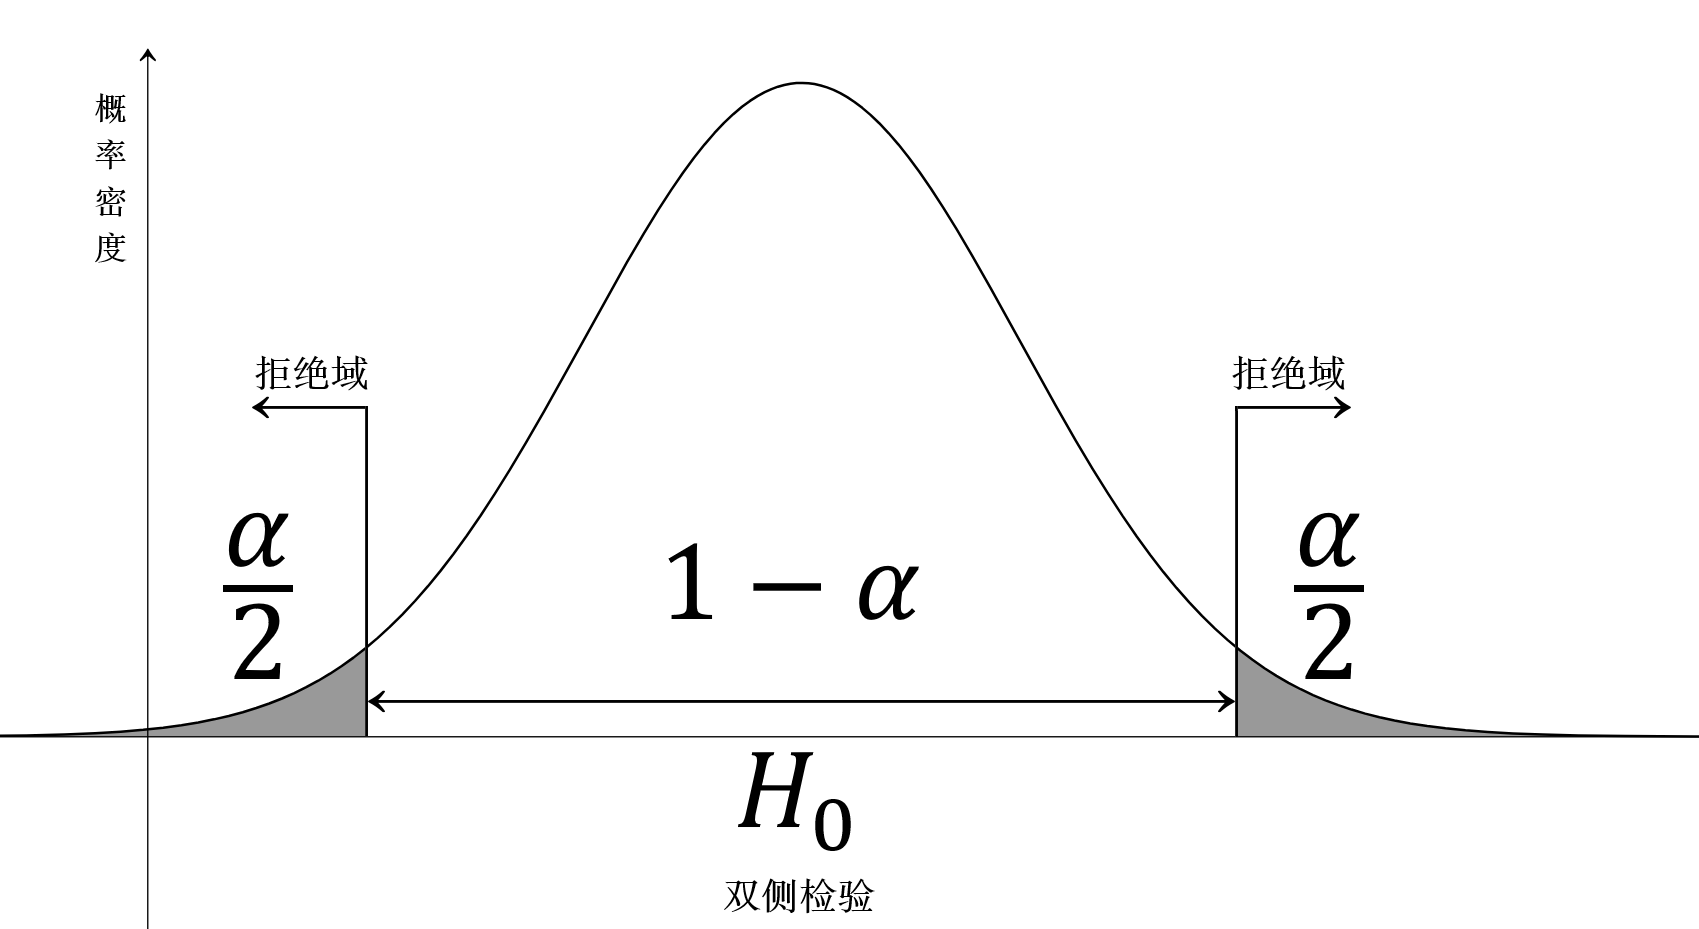
\includegraphics[width=0.6\linewidth]{BilateralTesting.png}
    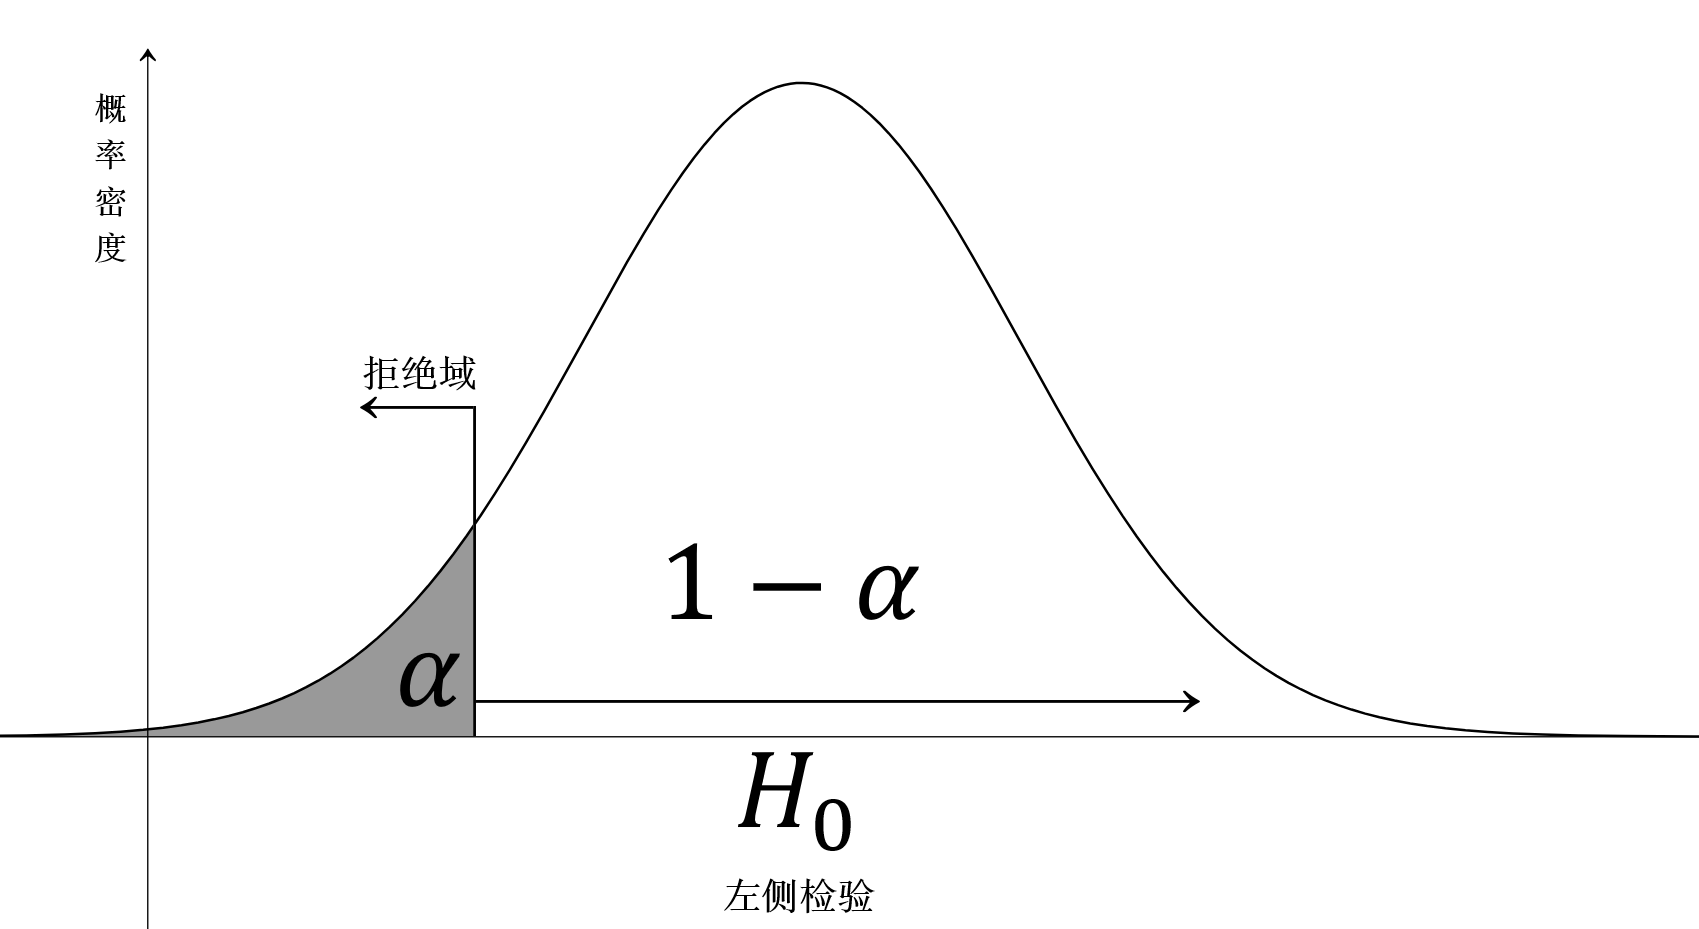
\includegraphics[width=0.6\linewidth]{LeftSideTest.png}
    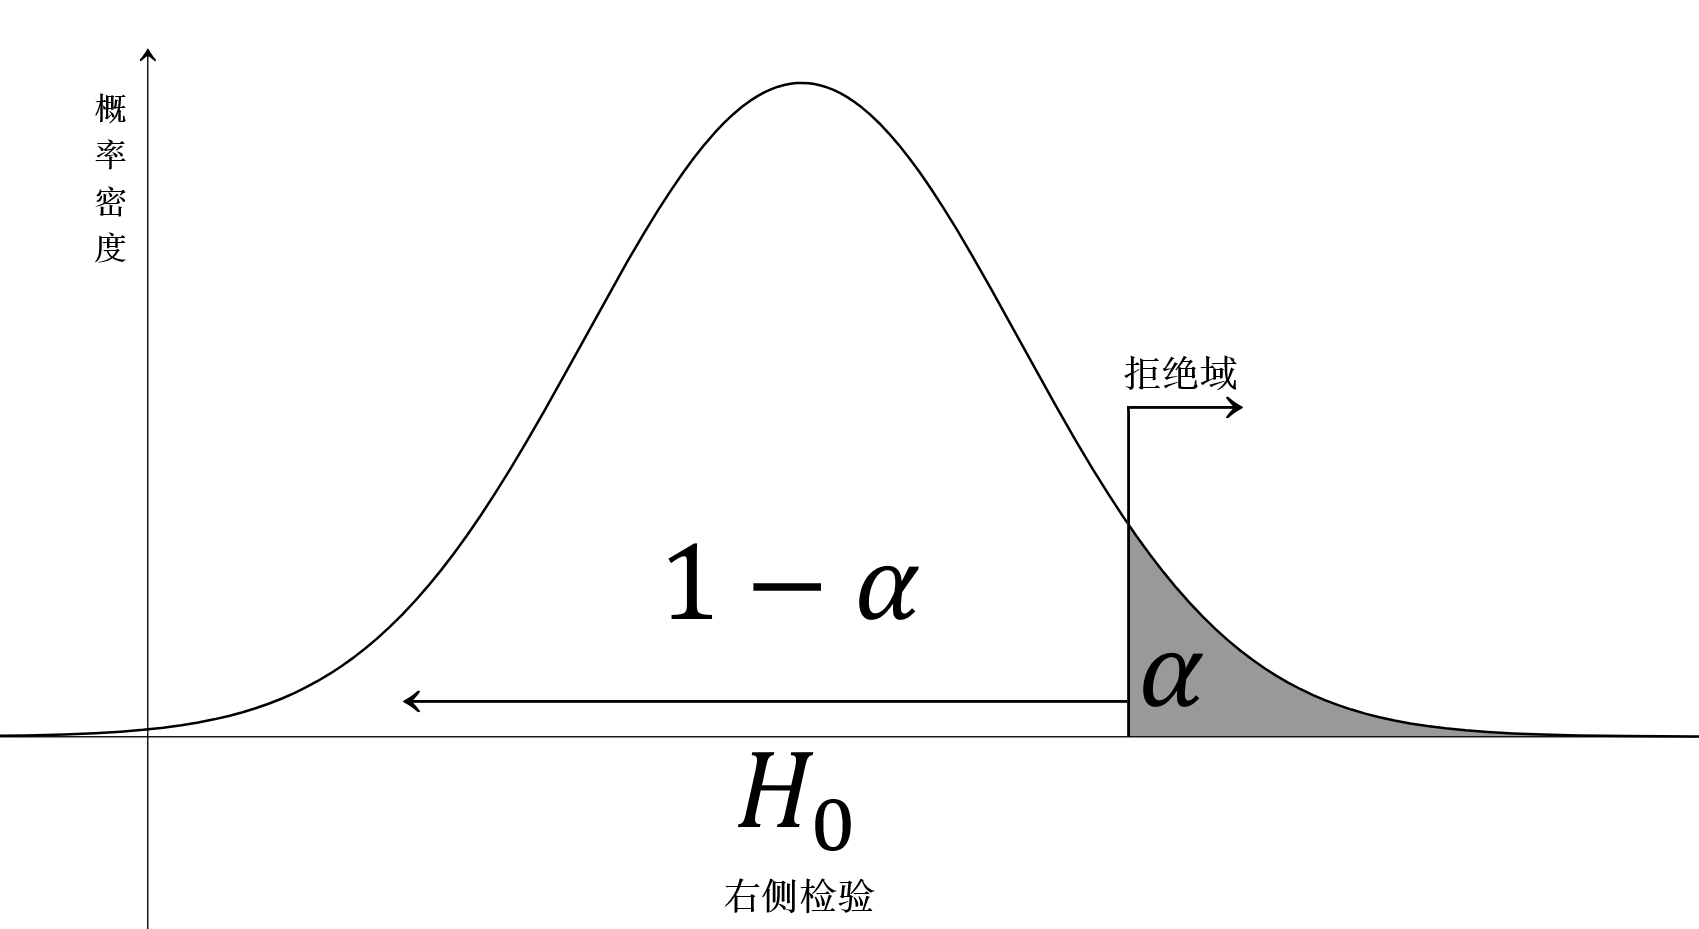
\includegraphics[width=0.6\linewidth]{RightSideTest.png}
\end{figure}

\newpage

\appendix

\part{附录}

\section{正态总体的常用统计量分布}

\subsection{单个正态总体的抽样分布}

\[\begin{aligned}
        X_1,X_2,\cdots,X_n                                                 & \sim N\p{\mu,\sigma^2}         \\
                                                                           & \Downarrow                     \\
        \bar X,S^2                                                         & \text{相互独立}                    \\
        \bar X                                                             & \sim N\p{\mu,\frac{\sigma^2}n} \\
        \bar X^\ast                                                        & \sim N\p{0,1}                  \\
        \sumin X_i^{\ast2}                                                 & \sim\chi^2\p{n}                \\
        \frac{\p{n-1}S^2}{\sigma^2}=\frac1{\sigma^2}\sumin\p{X_i-\bar X}^2 & \sim\chi^2\p{n-1}              \\
        \frac{\bar X-\mu}{S/\sqrt n}                                       & \sim t\p{n-1}                  \\
    \end{aligned}\]

\subsection{两个正态总体的抽样分布}

\[\begin{aligned}
        X_1,X_2,\cdots,X_m                                                                                                     & \sim N\p{\mu_X,\sigma_X^2}                                    \\
        Y_1,Y_2,\cdots,Y_n                                                                                                     & \sim N\p{\mu_Y,\sigma_Y^2}                                    \\
        \text{且两个样本相互独立}                                                                                                       & \Downarrow                                                    \\
        \bar X\pm\bar Y                                                                                                        & \sim N\p{\mu_X\pm\mu_Y,\frac{\sigma_X^2}m+\frac{\sigma_Y^2}n} \\
        \p{\bar X\pm\bar Y}^\ast                                                                                               & \sim N\p{0,1}                                                 \\
        \frac{\p{m-1}S_X^2}{\sigma_X^2}+\frac{\p{n-1}S_Y^2}{\sigma_Y^2}                                                        & \sim\chi^2\p{m+n-2}                                           \\
        \frac{\sum\limits_{i=1}^mX_i^{\ast2}/m}{\sumin Y_i^{\ast2}/n}                                                          & \sim F\p{m,n}                                                 \\
        \frac{S_X^2/S_Y^2}{\sigma_X^2/\sigma_Y^2}                                                                              & \sim F\p{m-1,n-1}                                             \\
        \text{当}\sigma_X^2=\sigma_Y^2=\sigma^2                                                                                 & \text{时}                                                      \\
        \frac{\p{\bar X-\bar Y}-\p{\mu_X-\mu_Y}}{\sqrt{\dfrac{\p{m-1}S_X^2+\p{n-1}S_Y^2}{m+n-2}}\cdot\sqrt{\dfrac1m+\dfrac1n}} & \sim t\p{m+n-2}                                               \\
    \end{aligned}\]

\newpage

\section{正态总体相关表}

\begin{longtblr}[
        caption = {正态总体的区间估计枢轴变量和置信水平为$1-\alpha$的双侧置信区间},
        note{$\dagger$} = {$S_\omega=\sqrt{\dfrac{\p{m-1}S_X^2+\p{n-1}S_Y^2}{m+n-2}}$},
        note{$\ddagger$} = {对应参数未知时,用$\bar X$代替$\mu$,用$S^2$代替$\sigma^2$}
    ]{colspec={c|c|c|c|c},hlines,cells={valign=m}}
    \hline
    待估参数$\theta$                                     & 条件$T$                    & 枢轴变量$I$                                  & 服从分布$F$         & 双侧置信区间$\p{\hat\theta_1,\hat\theta_2}$                                                                               \\
    \hline
    \SetCell[r=2]{c}$\mu$                            & $\sigma^2$已知             & $\dfrac{\bar X-\mu}{\sigma/\sqrt n}$     & $N\p{0,1}$      & $\p{\bar X\pm\dfrac\sigma{\sqrt n}z_{\alpha/2}}$                                                                    \\
                                                     & $\sigma^2$未知             & $\dfrac{\bar X-\mu}{S/\sqrt n}$          & $t\p{n-1}$      & $\p{\bar X\pm\dfrac S{\sqrt n}t_{\alpha/2}\p{n-1}}$                                                                 \\
    \SetCell[r=2]{c}$\sigma^2$                       & $\mu$已知                  & $\dfrac1{\sigma^2}\sumin{\p{X_i-\mu}}^2$ & $\chi^2\p{n}$   & $\p{\dfrac{\sumin{\p{X_i-\mu}}^2}{\chi_{\alpha/2}^2\p{n}},\dfrac{\sumin{\p{X_i-\mu}}^2}{\chi_{1-\alpha/2}^2\p{n}}}$ \\
                                                     & $\mu$未知                  & $\dfrac{\p{n-1}S^2}{\sigma^2}$           & $\chi^2\p{n-1}$ & $\p{\dfrac{\p{n-1}S^2}{\chi_{\alpha/2}^2\p{n-1}},\dfrac{\p{n-1}S^2}{\chi_{1-\alpha/2}^2\p{n-1}}}$                   \\
    \hline
    \SetCell[r=2]{c}$\mu_X-\mu_Y$                    & {$\sigma_X^2,\sigma_Y^2$                                                                                                                                                                                    \\已知}          & $\dfrac{\p{\bar X-\bar Y}-\p{\mu_X-\mu_Y}}{\sqrt{\dfrac{\sigma_X^2}m+\dfrac{\sigma_Y^2}n}}$  & $N\p{0,1}$      & $\p{\bar X-\bar Y\pm z_{\alpha/2}\sqrt{\dfrac{\sigma_X^2}m+\dfrac{\sigma_Y^2}n}}$    \\
                                                     & {$\sigma_X^2,\sigma_Y^2$                                                                                                                                                                                    \\未知}          & $\dfrac{\p{\bar X-\bar Y}-\p{\mu_X-\mu_Y}}{S_\omega\cdot\sqrt{\dfrac1m+\dfrac1n}}$           & $t\p{m+n-2}$    & {$\left(\bar X-\bar Y\pm\right.$\\$\left.t_{\alpha/2}\p{m+n-2}S_\omega\cdot\sqrt{\dfrac1m+\dfrac1n}\right)$}  \\
    \SetCell[r=2]{c}$\dfrac{\sigma_X^2}{\sigma_Y^2}$ & {$\mu_X,\mu_Y$                                                                                                                                                                                              \\已知}                    & $\dfrac{\sum\limits_{i=1}^m\p{X_i-\mu_X}^2/m\sigma_X^2}{\sumin\p{Y_i-\mu_Y}^2/n\sigma_Y^2}$  & $F\p{m,n}$      & {$\left(\dfrac{\dfrac1m\sum\limits_{i=1}^m\p{X_i-\mu_X}^2}{\dfrac1n\sumin\p{Y_i-\mu_Y}^2F_{\alpha/2}\p{m,n}},\right.$\\$\left.\dfrac{\dfrac1m\sum\limits_{i=1}^m\p{X_i-\mu_X}^2}{\dfrac1n\sumin\p{Y_i-\mu_Y}^2F_{1-\alpha/2}\p{m,n}}\right)$}  \\
                                                     & {$\mu_X,\mu_Y$                                                                                                                                                                                              \\未知}                    & $\dfrac{S_X^2/S_Y^2}{\sigma_X^2/\sigma_Y^2}$                                                 & $F\p{m-1,n-1}$  & {$\left(\dfrac{S_X^2}{S_Y^2}\cdot\dfrac1{F_{\alpha/2}\p{m-1,n-1}},\right.$\\$\left.\dfrac{S_X^2}{S_Y^2}\cdot\dfrac1{F_{1-\alpha/2}\p{m-1,n-1}}\right)$}                                                                                   \\
    \hline
\end{longtblr}

\newpage

\begin{longtblr}[
        caption = {正态总体的假设检验检验统计量和置信水平为$1-\alpha$的拒绝域},
        note{$\dagger$} = {$S_\omega=\sqrt{\dfrac{\p{m-1}S_X^2+\p{n-1}S_Y^2}{m+n-2}}$},
        note{$\ddagger$} = {对应参数未知时,用$\bar X$代替$\mu$,用$S^2$代替$\sigma^2$}
    ]{colspec={c|c|c|c|c},hlines,cells={valign=m}}
    \hline
    原假设$H_0$                        & 条件$T$                                    & 检验统计量$I$                                                          & 服从分布$F$                         & 拒绝域$W$                                      \\
    \hline
    $\mu=\mu_0$                     & \SetCell[r=3]{c}$\sigma^2$已知             & \SetCell[r=3]{c}$U=\dfrac{\bar X-\mu_0}{\sigma/\sqrt n}$          & \SetCell[r=3]{c}$N\p{0,1}$      & $\abs u\geqslant u_{\alpha/2}$              \\
    $\mu\leqslant\mu_0$             &                                          &                                                                   &                                 & $u\geqslant u_{\alpha}$                     \\
    $\mu\geqslant\mu_0$             &                                          &                                                                   &                                 & $u\leqslant-u_{\alpha}$                     \\
    $\mu=\mu_0$                     & \SetCell[r=3]{c}$\sigma^2$未知             & \SetCell[r=3]{c}$T=\dfrac{\bar X-\mu_0}{S/\sqrt n}$               & \SetCell[r=3]{c}$t\p{n-1}$      & $\abs t\geqslant t_{\alpha/2}\p{n-1}$       \\
    $\mu\leqslant\mu_0$             &                                          &                                                                   &                                 & $t\geqslant t_{\alpha}\p{n-1}$              \\
    $\mu\geqslant\mu_0$             &                                          &                                                                   &                                 & $t\leqslant-t_{\alpha}\p{n-1}$              \\
    $\sigma^2=\sigma_0^2$           & \SetCell[r=3]{c}$\mu$已知                  & \SetCell[r=3]{c}$\chi^2=\dfrac1{\sigma_0^2}\sumin{\p{X_i-\mu}}^2$ & \SetCell[r=3]{c}$\chi^2\p{n}$   & {$\chi^2\geqslant\chi_{\alpha/2}^2\p{n}$或   \\$\chi^2\leqslant\chi_{1-\alpha/2}^2\p{n}$}     \\
    $\sigma^2\leqslant\sigma_0^2$   &                                          &                                                                   &                                 & $\chi^2\geqslant\chi_{\alpha}^2\p{n}$       \\
    $\sigma^2\geqslant\sigma_0^2$   &                                          &                                                                   &                                 & $\chi^2\leqslant\chi_{1-\alpha}^2\p{n}$     \\
    $\sigma^2=\sigma_0^2$           & \SetCell[r=3]{c}$\mu$未知                  & \SetCell[r=3]{c}$\chi^2=\dfrac{\p{n-1}S^2}{\sigma_0^2}$           & \SetCell[r=3]{c}$\chi^2\p{n-1}$ & {$\chi^2\geqslant\chi_{\alpha/2}^2\p{n-1}$或 \\$\chi^2\leqslant\chi_{1-\alpha/2}^2\p{n-1}$} \\
    $\sigma^2\leqslant\sigma_0^2$   &                                          &                                                                   &                                 & $\chi^2\geqslant\chi_{\alpha}^2\p{n-1}$     \\
    $\sigma^2\geqslant\sigma_0^2$   &                                          &                                                                   &                                 & $\chi^2\leqslant\chi_{1-\alpha}^2\p{n-1}$   \\
    \hline
    $\mu_X-\mu_Y=\delta$            & \SetCell[r=3]{c}{$\sigma_X^2,\sigma_Y^2$                                                                                                                                                     \\已知} & \SetCell[r=3]{c}$U=\dfrac{\p{\bar X-\bar Y}-\delta}{\sqrt{\dfrac{\sigma_X^2}m+\dfrac{\sigma_Y^2}n}}$ & \SetCell[r=3]{c}$N\p{0,1}$      & $\abs u\geqslant u_{\alpha/2}$              \\
    $\mu_X-\mu_Y\leqslant\delta$    &                                          &                                                                   &                                 & $u\geqslant u_{\alpha}$                     \\
    $\mu_X-\mu_Y\geqslant\delta$    &                                          &                                                                   &                                 & $u\leqslant-u_{\alpha}$                     \\
    $\mu_X-\mu_Y=\delta$            & \SetCell[r=3]{c}{$\sigma_X^2,\sigma_Y^2$                                                                                                                                                     \\未知} & \SetCell[r=3]{c}$T=\dfrac{\p{\bar X-\bar Y}-\delta}{S_\omega\cdot\sqrt{\dfrac1m+\dfrac1n}}$          & \SetCell[r=3]{c}$t\p{m+n-2}$    & $\abs t\geqslant t_{\alpha/2}\p{m+n-2}$     \\
    $\mu_X-\mu_Y\leqslant\delta$    &                                          &                                                                   &                                 & $t\geqslant t_{\alpha}\p{m+n-2}$            \\
    $\mu_X-\mu_Y\geqslant\delta$    &                                          &                                                                   &                                 & $t\leqslant-t_{\alpha}\p{m+n-2}$            \\
    $\sigma_X^2=\sigma_Y^2$         & \SetCell[r=3]{c}{$\mu_X,\mu_Y$                                                                                                                                                               \\已知}           & \SetCell[r=3]{c}$F=\dfrac{\sum\limits_{i=1}^m\p{X_i-\mu_X}^2/m}{\sumin\p{Y_i-\mu_Y}^2/n}$            & \SetCell[r=3]{c}$F\p{m,n}$      & {$F\geqslant F_{\alpha/2}\p{m,n}$或          \\$F\leqslant F_{1-\alpha/2}\p{m,n}$}     \\
    $\sigma_X^2\leqslant\sigma_Y^2$ &                                          &                                                                   &                                 & $F\geqslant F_{\alpha}\p{m,n}$              \\
    $\sigma_X^2\geqslant\sigma_Y^2$ &                                          &                                                                   &                                 & $F\leqslant F_{1-\alpha}\p{m,n}$            \\
    $\sigma_X^2=\sigma_Y^2$         & \SetCell[r=3]{c}{$\mu_X,\mu_Y$                                                                                                                                                               \\未知}           & \SetCell[r=3]{c}$F=\dfrac{S_X^2}{S_Y^2}$                                                             & \SetCell[r=3]{c}$F\p{m-1,n-1}$  & {$F\geqslant F_{\alpha/2}\p{m-1,n-1}$或      \\$F\leqslant F_{1-\alpha/2}\p{m-1,n-1}$} \\
    $\sigma_X^2\leqslant\sigma_Y^2$ &                                          &                                                                   &                                 & $F\geqslant F_{\alpha}\p{m-1,n-1}$          \\
    $\sigma_X^2\geqslant\sigma_Y^2$ &                                          &                                                                   &                                 & $F\leqslant F_{1-\alpha}\p{m-1,n-1}$        \\
    \hline
\end{longtblr}

\end{document}
